\renewcommand{\figurename}{}
\mychapter{R307 Réseaux d'accès (24h)}{cap:r307}
\lhead{R307 Réseaux d'accès (24h)}

\vspace*{0.2cm}
      \large
      \href{\@orientadorPagina}{\color{black}Enseignant\\Mr. Yannick Lespine}\\
\vspace*{0.5cm}

Enseignement délivré sur la première période à l'IUT. Ce module avait pour objectif de nous faire apprendre les technologies des réseaux d'accès des FAI \textit{Fournisseur d'Accès Internet}. Celui-ci est lié au module R302 et les réseaux d'opérateurs, aussi appelés réseaux backbone. Ce module a un fort coefficient dans la deuxième compétence télécommunications. Nous y avons étudié en profondeur les technologies xDSL, et appliqué certains principes réseaux comme le DHCP, le NAT et d'autres.

\section{Apprentissage théorique des réseaux à technologie xDSL}

Lors des cours et des travaux dirigés, nous avons intégré le fonctionnement des réseaux d'accès à technologie xDSL \textit{Digital Subscriber Line}. Basés sur le réseau téléphonique déjà existant, les technologies xDSL avaient comme objectif de l'utiliser pour raccorder des abonnées à Internet, en plus d'accéder à la téléphonie. De là sont nés l'ADSL \textit{Asymetric DSL} GDMT, 2 et 2+ ou encore la VDSL \textit{Very high-speed Digital Subscriber Lines}.
\\ \\
L'ADSL est la technologie que nous avons le plus abordé. Celle-ci est présente dans sa plus ancienne version, GDMT, jusqu'à la dernière l'ADSL2+. Ces deux possèdent des spectres conservant la déontologie des spectres de réseau ADSL : une bande passante pour le POTS \textit{Plain Old Telephone Service (la téléphonie)}, une autre pour le flux sortant et une plus grande pour le flux rentrant (car abonné consommateur de services sur Internet, pas producteur).

\begin{figure}[h]
    \centering
    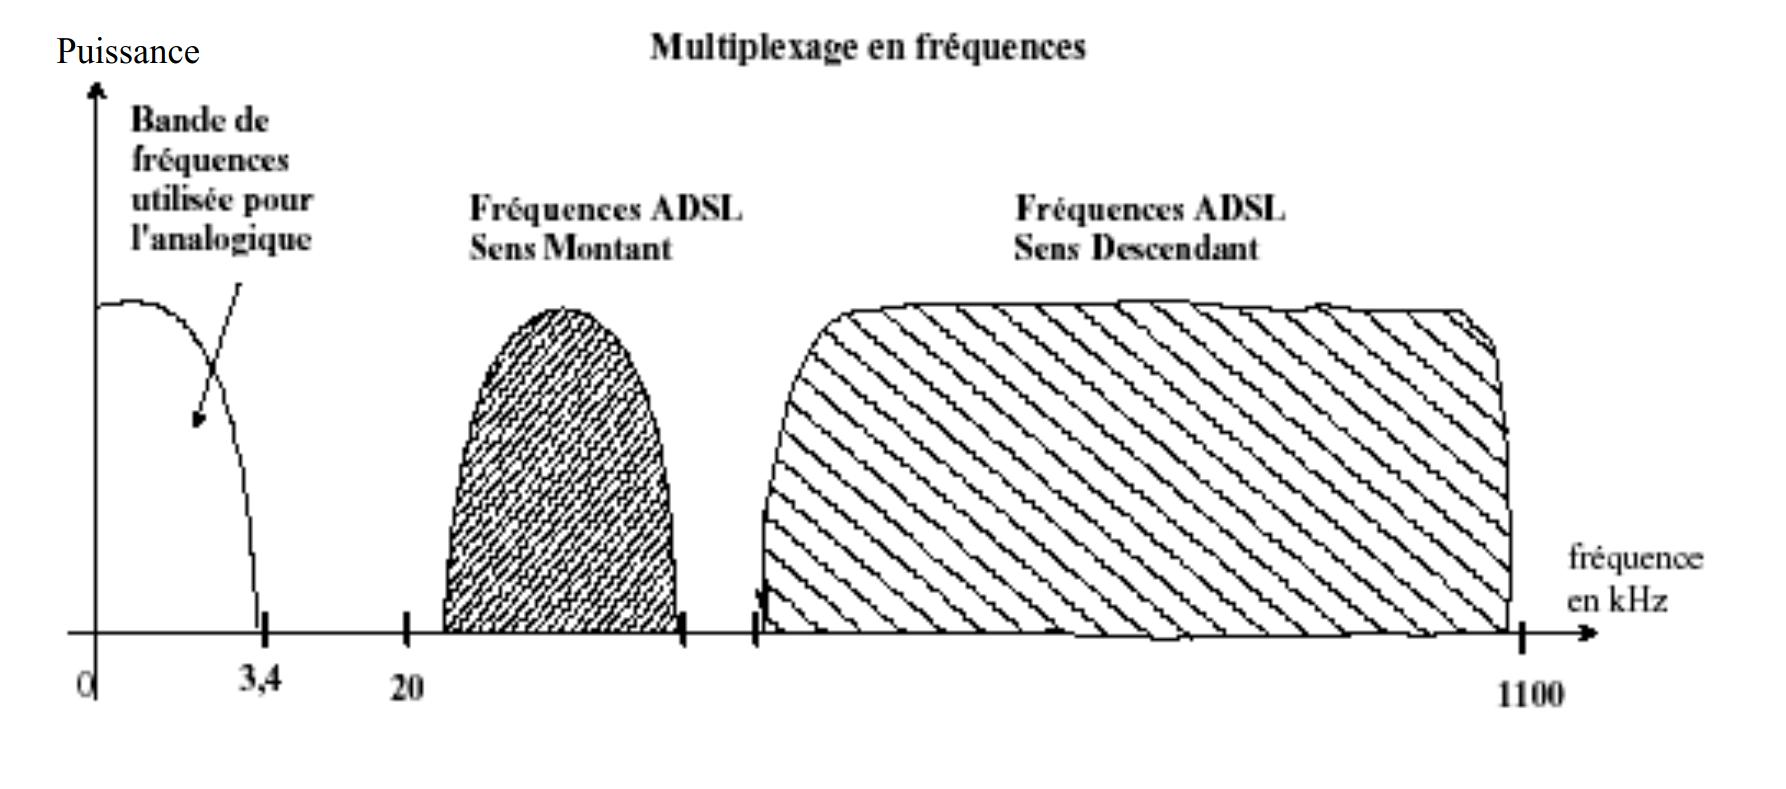
\includegraphics[width=1\linewidth]{imgs/tmp_adsl.jpg}
    \caption{Spectre d'amplitude d'un lien ADSL}
    \label{fig:tmp_adsl}
\end{figure}

L'ADSL utilise une modulation dans son signal pour tirer le meilleur débit possible de ses bandes passantes. Nous avons revu les types de modulation, sans aborder dans les détails la modulation DMT \textit{Discrete MultiTone} de l'ADSL. Nous avons aussi confirmé que le débit maximal pratique était définit par la distance qui nous reliée à l'équipement de l'opérateur. En effet, le support étant une paire de cuivre torsadée, celle-ci se comporte comme une résistance au passage du courant : elle augmente sa résistivité par la distance et le courant traversé. Les fréquences qui composent le signal reçoivent une atténuation de plus en plus forte proportionnellement à la distance, ce qui diminue leur valence, et donc le débit qu'elles peuvent faire transiter.
\\ \\
La modulation est gérée d'un côté par un modulateur et de l'autre par un démodulateur. Ce mécanisme fonctionne pour une communication dans un sens (celui qui envoie n'est pas celui qui reçoit). Pour que les deux côtés puissent envoyer et recevoir des informations, ont été conçu les modems - abrévation pour modulateur/démodulateur. L'équipement chargé de cette action chez le FAI est le DSLAM \textit{Digital Subscriber Line Access Multiplexer} qui s'occupent de rattacher les équipements abonnés au réseau backbone opérateur pour accéder à internet, et le modem chez le client pour envoyer des informations selon la même modulation au DSLAM, et démoduler celles reçues.
\\ \\
Nous avons aussi beaucoup étudié les couches protocolaires, comme le fonctionnement du protocole ATM \textit{Asynchronous Transfer Mode} et ses cellules, aisni que ses protocoles de couches supérieures. Nous avions ainsi toutes les informations nécéssaires, et plus, pour comprendre le type de topologie ci dessous.

\begin{figure}[h]
    \centering
    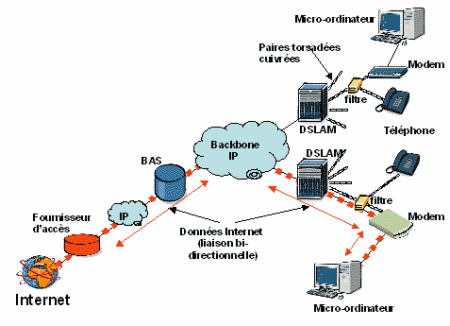
\includegraphics[width=1\linewidth]{imgs/tmp_adsl2.png}
    \caption{Schéma d'une liaison opérateur FAI et abonné en ADSL}
    \label{fig:tmp_adsl2}
\end{figure}

Le BAS \textit{Broadband Access Server} est un serveur permetant l'authentification des abonnées par l'utilisation de protocoles comme le PPPoE \textit{Point-to-Point Protocol over Ethernet} sur la couche ethernet ou le PPPoA \textit{PPPo ATM} sur la couche ATM. Auquel cas n'importe qu'elle personne, sans abonnement, pourrait se rattacher au DSLAM par un port téléphonique raccordé et récupérer une adresse IP pour avoir accès à Internet. Ce serveur authentifie les abonnées auprès de l'opérateur, permettant la réception d'une adresse IP et leur accès à Internet \& aux services globales de l'opérateur.

\section{Projet d'étude d'un réseau d'accès ADSL}

Lors des travaux pratiques, nous avons pu mettre en place et caractériser un réseau à technologie ADSL. À l'issue de ce projet, nous avions un rapport globale à rendre et une présentation à soutenir. Les travaux pratiques constituent la moitié du temps consacré à ce module (12h).
\\ \\
Les premières séances de ce projet étaient dédiées à la prise en main des équipements mis à disposition et à la compréhension l'infrastructure de la salle. Ainsi, nous avons pris en main un modem et routeur Zyxel VMG1312-B10D pour l'équipement abonnée, un DSLAM ADSL IES 1000 côté opérateur, un testeur de ligne xDSL SUNRISE TELECOM MTT LITE DSL, des routeurs Cisco 2901 pour simuler l'arrière du réseau opérateur, et le réseau de la salle.
\\ \\
Nous avons abordé des notions plus en profondeur qu'en cours, en poussant notre étude pour comprendre le fonctionnement d'outils ou de notions annexes (diaphonie, synchronisation ADSL...). Nous avons lors de ce projet caractérisé une ligne ADSL via le testeur de ligne et interprété ses valeurs. Nous avons configuré les équipements de réseaux conformément aux apprentissages demandés (côté opérateur et abonné) afin de comprendre les différents types de topologies, pourquoi certaines comme celle en pont ne sont plus utilisés... Des protocoles, couches ou notions annexes ont aussi été abordé comme le DHCP dans le LAN et côté opérateur, la gestion de l'authentification par le protocole PPP, monter - caractériser \& différencier les types de NAT...
\\ \\
Le rapport de ce projet est disponible sur \href{https://karuta.univ-pau.fr/karuta-backend/resources/resource/file/1e82435e-9d2d-11ee-a8e6-aae0820000f2?lang=fr&timestamp=1706858357601https://karuta.univ-pau.fr/karuta-backend/resources/resource/file/1e82435e-9d2d-11ee-a8e6-aae0820000f2?lang=fr&timestamp=1706858357601}{Karuta}, les notes et le coefficient de ce module en annexe.

\section{Aboutissants du module}

Par ce module et particulièrement son projet intégratif, nous avons pu monter et étudier un réseau opérateur-abonné. Enseignement extrêmement intéressant, regroupant réseaux et télécommunications pour nous faire apprendre les différentes technologies les composants encore aujourd'hui. Les appliquer sur des équipements particuliers a aussi été très enrichissant pour l'utilisation d'outils tiers.